\addcontentsline{toc}{chapter}{Introducci\'on}

% Titulo de la introduccion.
\begin{center}
	{\bf Introducción} \label{chap:intro}
\end{center}

% Contenido de la introduccion.

\label{sect:motivacion}
%Puedes quitar esto(es opcional)
\vspace{5 mm}

En la Universidad Sim\'on Bol\'ivar es dictada la materia electiva
Dise\~no de Algoritmos II, en la cual se enseñan diversas metaheur\'isticas.
El curso es dividido en grupos (normalmente en parejas) y a cada uno se le asigna un problema 
de optimizaci\'on NP-hard para resolver mediante estos m\'etodos. Uno de \'estos es Data Clustering.
Consiste m\'etodo de crear grupos de objetos,
de tal manera que los objetos dentro de un cluster sean similares y 
en clusters distintos sean diferentes. \cite{GaChJi2007}

Este problema tiene las siguiente caracte\'isticas a considerar: \cite{SwAjAm2009}

\begin{itemize}

\item Hay muchas definciones porpuestas por una diversa cantidad de personas,
 lo que demuestra la dificultad de proveer una \'unica definici\'on formal. Ésto radica en que
no existe un criterio individual que se acerque a la noci\'on que tiene un humano. 
El siguiente ejemplo va a poner en claro.

Considere los siguientes animales: oveja, perro, gato (mam\'iferos), gorri\'on, gaviota (aves),
v\'ivora, lagarto (rept\'iles), pez de colores, salmonete, tibur\'on azul (peces), y rana (anf\'ibio).
Para organizar estos animales en clusters, se tiene que definir un criterio. Por ello, si 
elejimos la manera como se reproducen, la oveja, perro, gato
y tibur\'on azul van a ser asignados al mismo cluster, mientras que el resto van a formar un segundo
(Figura \ref{fig:ejemplo1}).  En cambio, si el criterio es la existencia de pulmones, 
el pez de colores, el salmonete y el tibur\'on son
asignados al mismo cluster, mientras que el resto a otro (Figura \ref{fig:ejemplo2}).
Por otro lado, si el criterio es el ambiente
donde viven los animales, la oveja, perro, gato, gorri\'on, gaviota, v\'ivora y el lagarto van a formar un cluster
(viven fuera del agua), el pez de colores, salmonete y el tibur\'on azul van a formar un otro (viven afuera
del agua), y un tercero que va a contener a la rana, ya que puede vivir en los dos (Figura \ref{fig:ejemplo3}). 

\begin{figure}[htb]
\centering
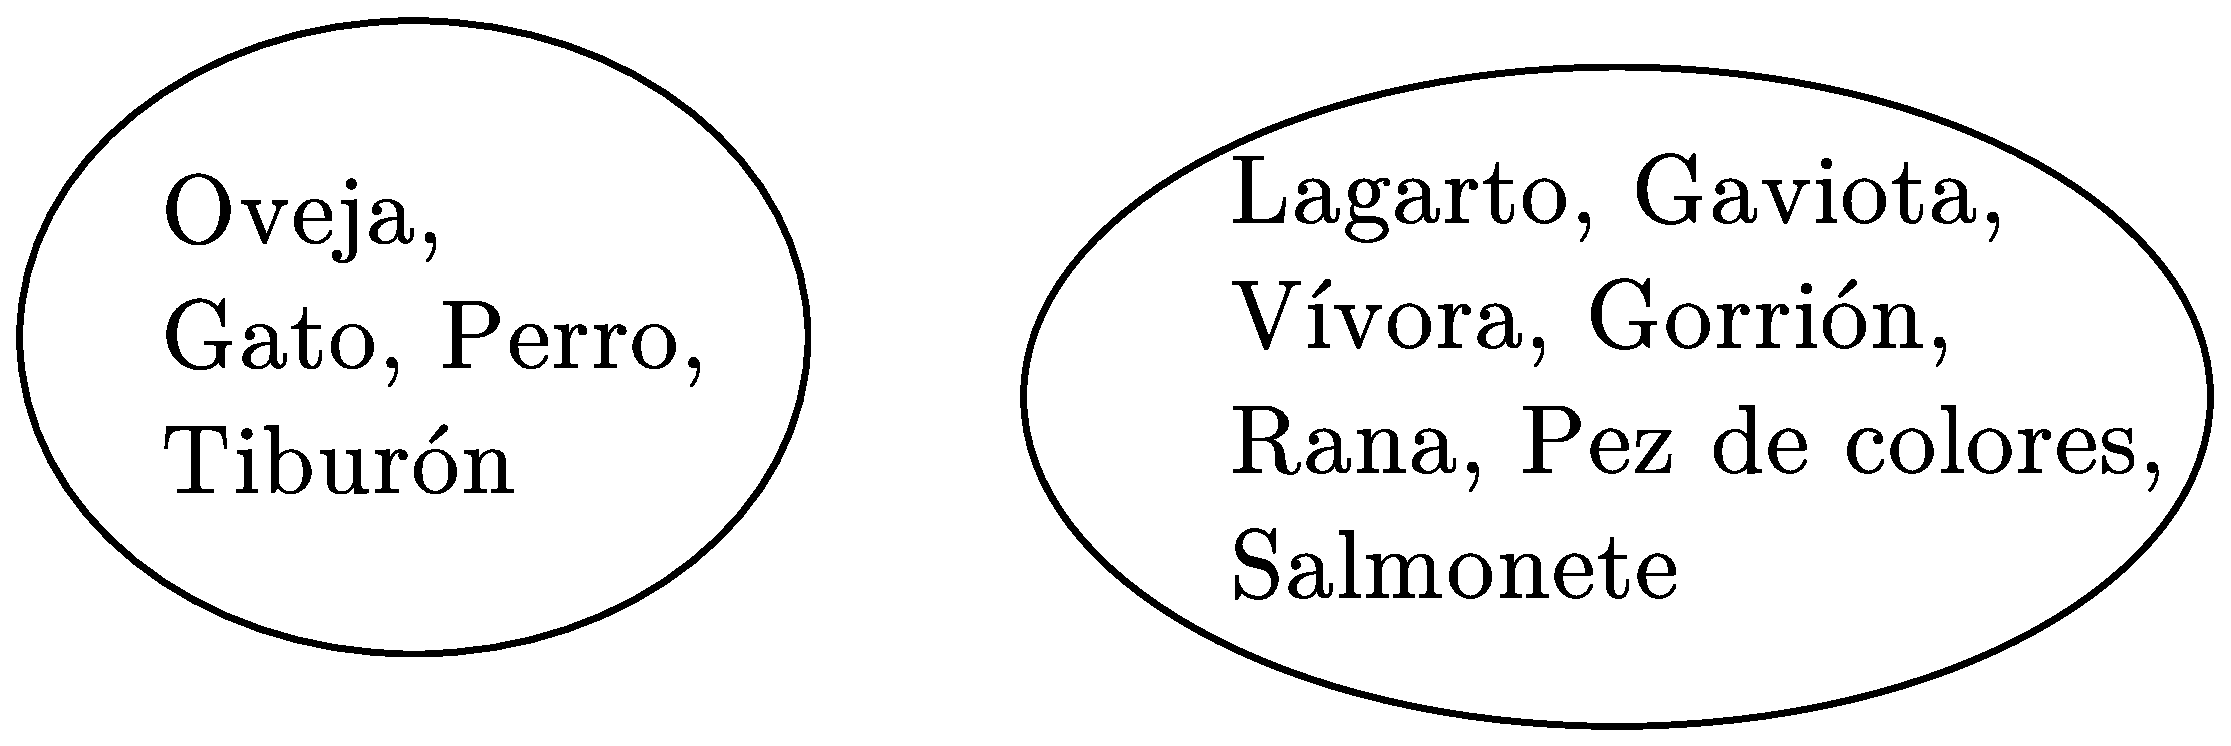
\includegraphics[scale=0.3]{figures/ejemplo1.eps}
\caption{Clustering usando como criterio la forma como se reproducen}
\label{fig:ejemplo1}
\end{figure}

\begin{figure}[htb]
\centering
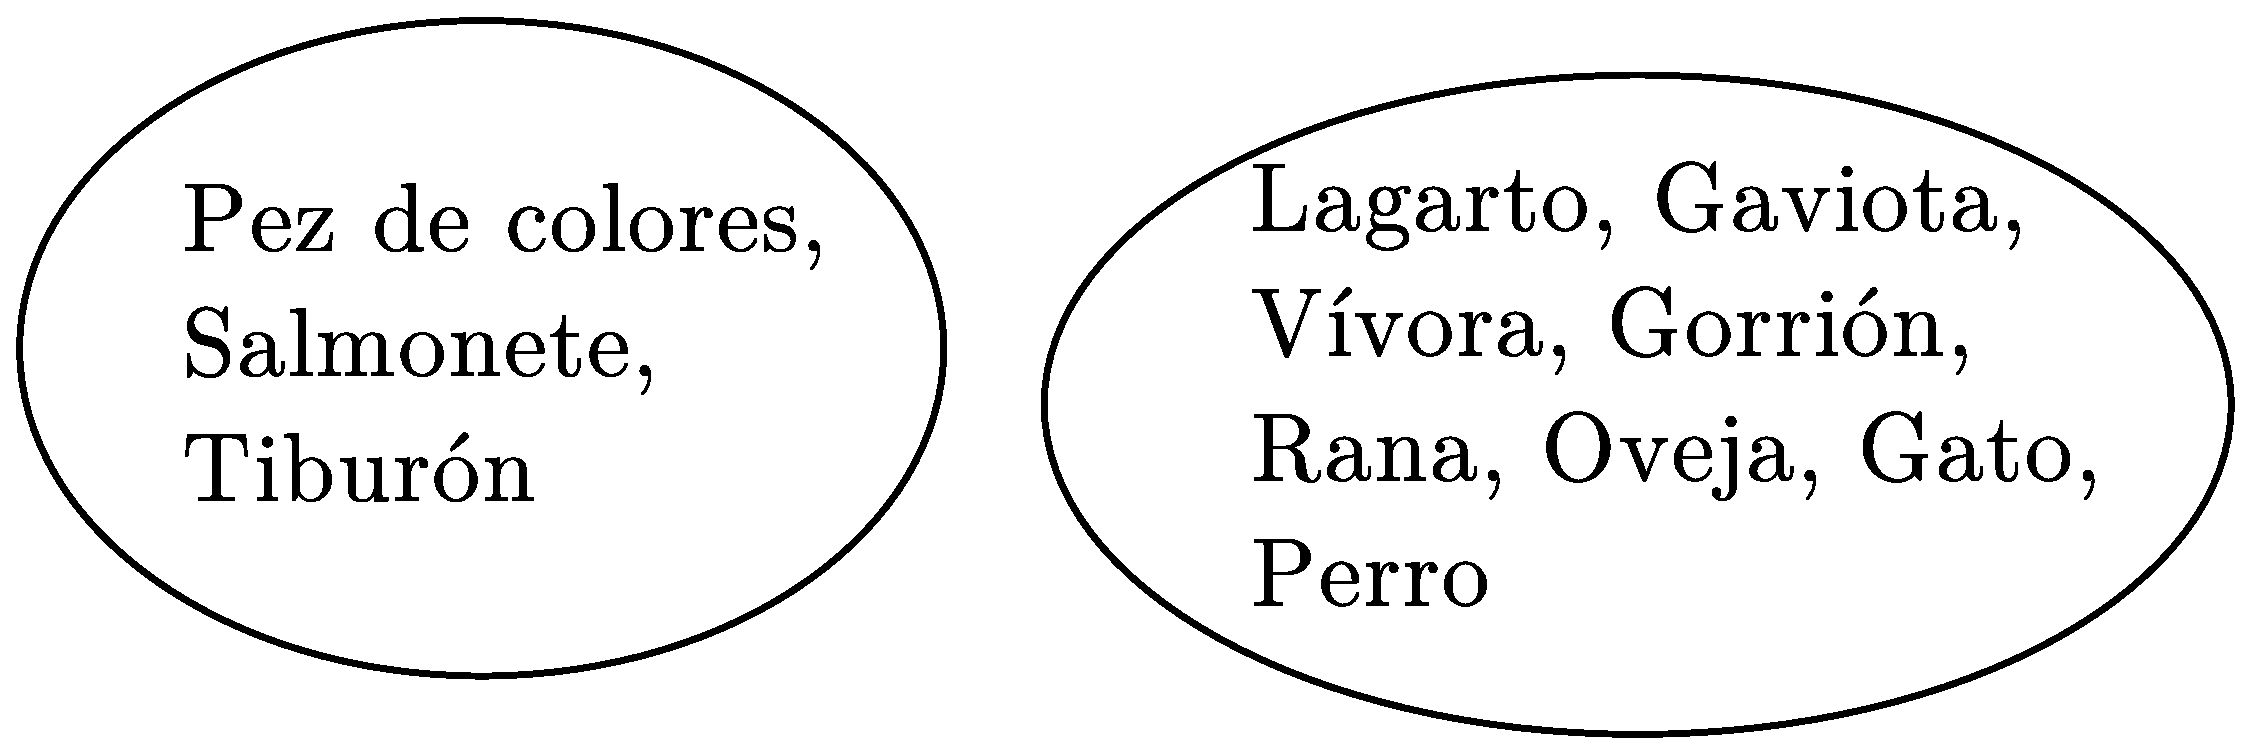
\includegraphics[scale=0.3]{figures/ejemplo2.eps}
\caption{Clustering usando como criterio la existencia de pulmones}
\label{fig:ejemplo2}
\end{figure}

\begin{figure}[htb]
\centering
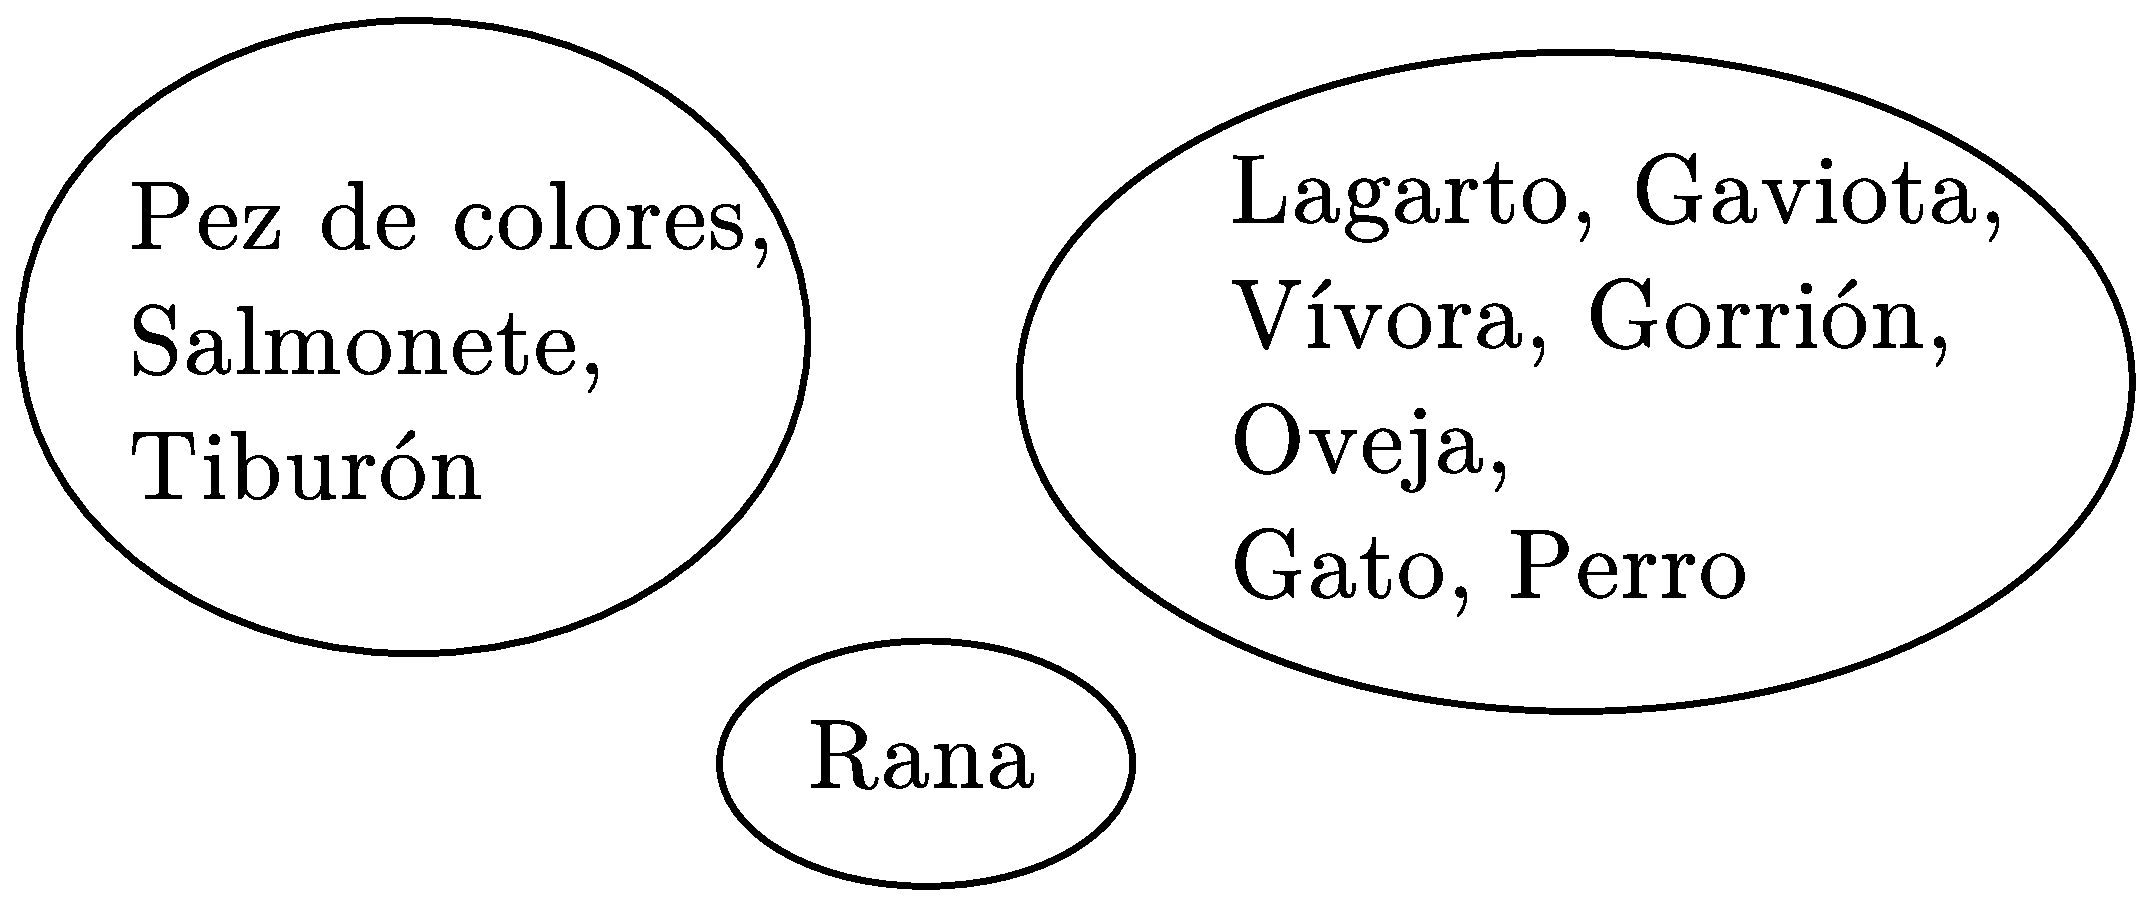
\includegraphics[scale=0.3]{figures/ejemplo3.eps}
\caption{Clustering usado como criterio el ambiente donde viven}
\label{fig:ejemplo3}
\end{figure}

Se puede ver que gracias a la falta de un criterio universal para el clustering,
 \'esta es muy subjetiva en muchos casos.

\item Se puede ver desde el punto de vista de aprendizaje autom\'atico, donde los clusters
correponden a patrones escondidos en los datos, la b\'usqueda de clusters 
es una especie de aprendizaje no supervisado. Es importante entender la diferencia
entre clustering (aprendizaje no supervisado) y clasificaci\'on supervisada. 
En esta \'ultima, se provee una colecci\'on patrones etiquetados
(preclasificados); el problema es etiquetar un patr\'on recien encontrado. 
Tipicamente, los patrones etiquetados (entrenamiento) ya son usados para obtener
las descripciones de las clases, que a su vez se utilizan para etiquetar un nuevo patr\'on.

En el caso de clustering, el problema consiste en agrupar una colecci\'on de patrones no etiquetados
en grupos significativos. En este sentidos, las etiquetas se asocian con los clusters tambi\'en,
pero esta categor\'ia de etiquetas est\'an basadas en datos, es decir, que se obtienen unicamente
de \'estos.

\item Un algoritmos de clustering se espera que descubra el agrupamiento natural
 que existe en una conjunto de patrones o puntos de datos. 
Cada patr\'on puede ser identificado como un punto en un hiperespacio,
llamado espacio de caracter\'isticas. La entrada
es un conjunto esos puntos en el espacio carater\'istico multidimensional. Un algoritmo ideal de 
clustering debe devolver como salida, la etiqueda para cada patr\'on, es decir,
el grupo al cual pertenece cada punto.

\end{itemize}

\'Este problema a sido abordado por diversos campos del conocimiento como la estad\'istica
(an\'aslisis multivariado), teor\'ia de grafos, computaci\'on evolutiva, redes neurales y
as\'i sucesivamente\cite{SwAjAm2009}. Entre sus aplicaciones se encuentra la miner\'ia de datos, 
segmentaciones de clientes y procesamiento de im\'agenes, entre otras. \cite{GaChJi2007}

En especial llama la atenci\'on el \'ultimo mencionado. El procesamiento de im\'agenes es muy \'util para los
humanos. Su importancia radica en que la salida de hacerle clustering a una imagen, puede ser usada como la entrada para 
un modelo basado en sistemas de reconocimiento de objetos.
\'Esto le da una gama de aplicaciones gigantescas: cualquier tipo de reconicimiento de im\'agenes.
Tambi\'en en el \'area m\'edica puede ayudar a encontrar regiones en las im\'agenes que sean de inter\'es,
que posiblemente humano no logre identificar.

Ejemplos son Google Goggles, diversos m\'odulos de JDownloader con el objetivo de reconocer
captchas, reconocimiento de caras por parte de las c\'amaras, el poder encontrar patrones escondido en
conjuntos de datos es muy \'util: una empresa podr\'ia mejorar su ventas, etc.

Brucker en \cite{Br1978} demotr\'o que el problema es NP-hard cuando el n\'umero 
de clusters excede 3.

%Puedes quitar esto(es opcional)
\vspace{5 mm}

\label{sect:planteamiento}
%Puedes quitar esto(es opcional)
\vspace{5 mm}

Actualmente existe una ardua investigaci\'on en diversas metaheur\'isticas para
resolver diversos problemas optimizaci\'on. La idea es obtener en un tiempo
considerable una respuesta \'optima o lo m\'as cercano posible a \'esta. Por
ello muchos cient\'ificos han empezado a inspirarse en la naturaleza.
Una profunda obsevaci\'on en la relaci\'on subyacente 
entre \'esta y optimizaci\'on ha llevado al desarrollo de nuevos paradigmas
para lograr este objetivo\cite{SwAjAm2009}. De ac\'a surgen las basadas en poblaci\'on e inteligencia
colectiva.

Los m\'as prominentes y prometedores son el algoritmo g\'enetico, abeja, DE, hormiga
y PSO. Todos constan de un grupo de individuos que van a ir modificandose a trav\'es
del tiempo. La forma en que se den estos cambios depende de cada algoritmo.

%Puedes quitar esto(es opcional)
\vspace{5 mm}

\label{sect:objetivo_general}
%Puedes quitar esto(es opcional)
\vspace{5 mm}

El objetivo principal es la implementaci\'on de \'estas cinco metaheur\'isticas
y el K-means, el algoritmo m\'as famoso para data clustering, para ver la calidad
de cada uno y compararlos entre si. \'Esta debe ser eficiente, rapida y flexible
con el objetivo de que pueda ser usada a futuro por otras personas y lograr
comprar los algoritmos de la forma m\'as efectiva.


%Puedes quitar esto(es opcional)
\vspace{5 mm}

\label{sect:objetivos_especificos}
%Puedes quitar esto(es opcional)
\vspace{5 mm}

El programa debe tener la capcidad de leer archivos en formato CSV e im\'agenes
en formato PNG y TIFF (las im\'agenes son datos n\'umericos). La salida tiene que ser
concorde al tipo de cada archivo, para un csv un archivo de texto y
en el otro caso una imagen con un color para cada grupo creado. Es necesario que
el lenguaje que se use tenga la capcidad de compilar a c\'odigo de m\'aquina
en vista que se busca eficiencia en tiempo.

Para comparar las diversas metaheur\'sticas es esencial tener una m\'etrica com\'un
con ese fin. Adem\'as se debe colocar un limite de tiempo en las corridas para 
obtener una buena soluci\'on en un tiempo considerable.


